
Šiame darbe yra palyginami 4 neuroninių tinklų architektūros: daugiavaizdis neuroninis tinklas, aprašytas poskyryje Daugiavaizdis konvoliucinis neuroninis tinklas, kapsulinis neuroninis tinklas, aprašytas poskyryje Tiriamo kapsulinio neuroninio tinklo architektūra, ir 2 daugiavaizdžiai kapsuliniai neuroniniai tinklai, aprašyti poskyriuose Tiriamo daugiavaizdžio kapsulinio neuroninio tinklo architektūra su vaizdų sujungimo sluoksniu ir Tiriamo daugiavaizdžio kapsulinio neuroninio tinklo architektūra su vaizdų kapsuliniu sluoksniu. Kiekvienas tiriamas dirbtinis neuroninis tinklas yra apmokomas naudojantis visais duomenimis, aprašytais poskyryje Tyrimams naudoti duomenys. Šie duomenys apmokymo metu yra padalinami į duomenų rinkinius, kurių dydžiai yra 96. Daugiavaizdžio konvoliucinio ir kapsulinio neuroninių tinklų apmokymų antram etapui duomenų rinkiniai buvo sudaryti iš nuotraukų grupių, kuriose yra visos konkretaus 3D objekto modelio nuotraukos. Kiekvienas dirbtinis neuroninis tinklas yra apmokomas per 10 epochų. Daugiavaizdžio konvoliucinio ir kapsulinio neuroninių tinklų abu apmokymo etapai yra apmokomi po 5 epochas.

Po kiekvienos epochos yra renkamos tikslumo metrikos: tikslumas klasifikuojant apmokymo duomenis, ši informacija pavaizduota lentelėje \ref{tbl:train} ir grafe \ref{img:train_plot}, ir tikslumas klasifikuojant testavimo duomenis, ši informacija atvaizduota lentelėje \ref{tbl:valid} ir grafe \ref{img:valid}. Tikslumas yra teisingai suklasifikuotų įrašų dalis klasifikuotų duomenų aibėje. Lentelių \ref{tbl:train}, \ref{tbl:valid} stulpelių pavaidinimai ir grafų \ref{img:train_plot}, \ref{img:val_plot} pavadinimai.

\begin{table}[]
\begin{tabular}{|l|l|l|l|l|l|}
	\hline
	epocha &     mvcnn &   capsnet & mv\_capsnet & mv\_cap\_capsnet1 & mv\_cap\_capsnet2 \\ \hline
	0 &  0.791531 &  0.302292 &   0.718333 &        0.479573 &        0.479573 \\ \hline
	1 &  0.835160 &  0.561875 &   0.768125 &        0.629025 &        0.629025 \\ \hline
	2 &  0.849466 &  0.630833 &   0.777917 &        0.687466 &        0.687466 \\ \hline
	3 &  0.857515 &  0.663125 &   0.783958 &        0.714421 &        0.714421 \\ \hline
	4 &  0.859916 &  0.683125 &   0.800417 &        0.721354 &        0.721354 \\ \hline
	5 &  0.888393 &  0.674167 &   0.800000 &        0.831981 &        0.831981 \\ \hline
	6 &  0.880276 &  0.698333 &   0.822500 &        0.848214 &        0.848214 \\ \hline
	7 &  0.881088 &  0.701250 &   0.827500 &        0.838068 &        0.838068 \\ \hline
	8 &  0.896104 &  0.722917 &   0.807500 &        0.840503 &        0.840503 \\ \hline
	9 &  0.900974 &  0.710417 &   0.852500 &        0.827516 &        0.827516 \\ \hline
	
\end{tabular}
\caption{
	Apmokymo duomenų klasifikavimo tikslumas, kur mvcnn yra daugiavaizdžio neuroninio tinklo tikslumas, capsnet - kapsulinio neuroninio tinklo tikslumas, mv\_capsnet - daugiavaizdžio kapsulinio neuroninio tinklo su , mv\_cap\_capsnet1 - , mv\_cap\_capsnet2
}
\label{tbl:train}
\end{table}

\begin{table}[]
	\begin{tabular}{|l|l|l|l|l|l|}
		\hline
		epocha &     mvcnn &   capsnet & mv\_capsnet & mv\_cap\_capsnet1 & mv\_cap\_capsnet2 \\ \hline
		0 &  0.791531 &  0.302292 &   0.718333 &        0.479573 &        0.479573 \\ \hline
		1 &  0.835160 &  0.561875 &   0.768125 &        0.629025 &        0.629025 \\ \hline
		2 &  0.849466 &  0.630833 &   0.777917 &        0.687466 &        0.687466 \\ \hline
		3 &  0.857515 &  0.663125 &   0.783958 &        0.714421 &        0.714421 \\ \hline
		4 &  0.859916 &  0.683125 &   0.800417 &        0.721354 &        0.721354 \\ \hline
		5 &  0.888393 &  0.674167 &   0.800000 &        0.831981 &        0.831981 \\ \hline
		6 &  0.880276 &  0.698333 &   0.822500 &        0.848214 &        0.848214 \\ \hline
		7 &  0.881088 &  0.701250 &   0.827500 &        0.838068 &        0.838068 \\ \hline
		8 &  0.896104 &  0.722917 &   0.807500 &        0.840503 &        0.840503 \\ \hline
		9 &  0.900974 &  0.710417 &   0.852500 &        0.827516 &        0.827516 \\ \hline
		
	\end{tabular}
	\caption{Daugiavaizdis konvoliucinis neuroninis tinklas}
	\label{tbl:valid}
\end{table}

\begin{figure}[H]
	\centering
	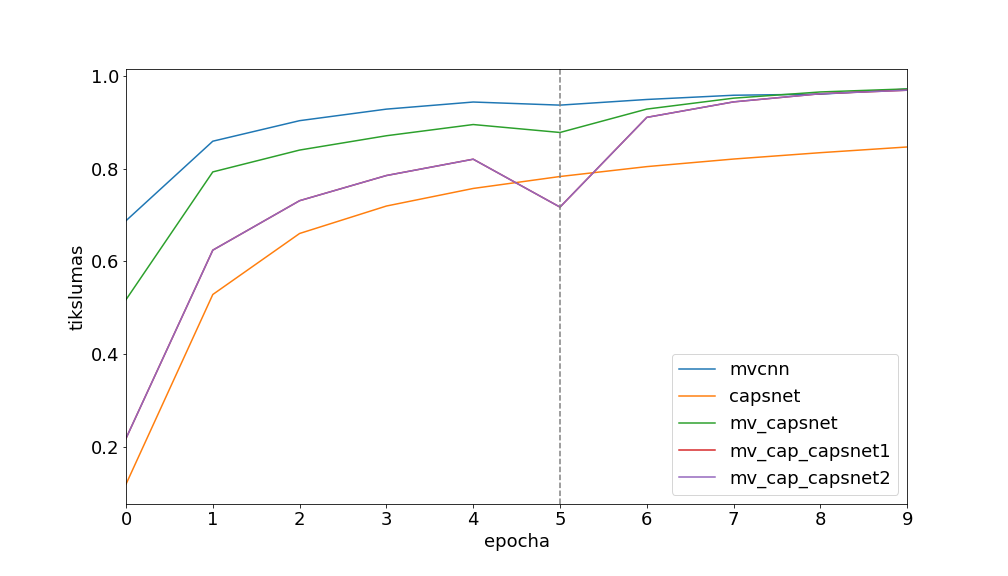
\includegraphics[scale=0.5]{img/trained.png}
	\caption{Daugiavaizdis konvoliucinis neuroninis tinklas}
	\label{img:train_plot}
\end{figure}

\begin{figure}[H]
	\centering
	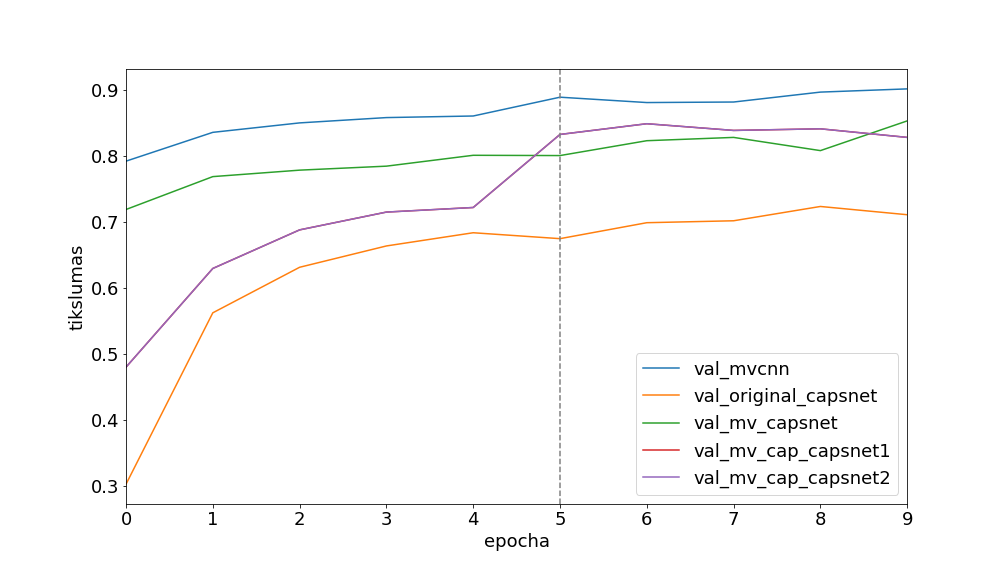
\includegraphics[scale=0.5]{img/validated.png}
	\caption{Daugiavaizdis konvoliucinis neuroninis tinklas}
	\label{img:val_plot}
\end{figure}
